%!TEX root = ../thesis.tex

\section{Shrinking chords}
In this section we will explain the operation of \emph{shrinking chords}.


Suppose that during sweeping we find a chord  in our candidate walk. Then we are in the situation of Figure \ref{fig:chord:situation}.

\begin{figure}[h]
  \centering
  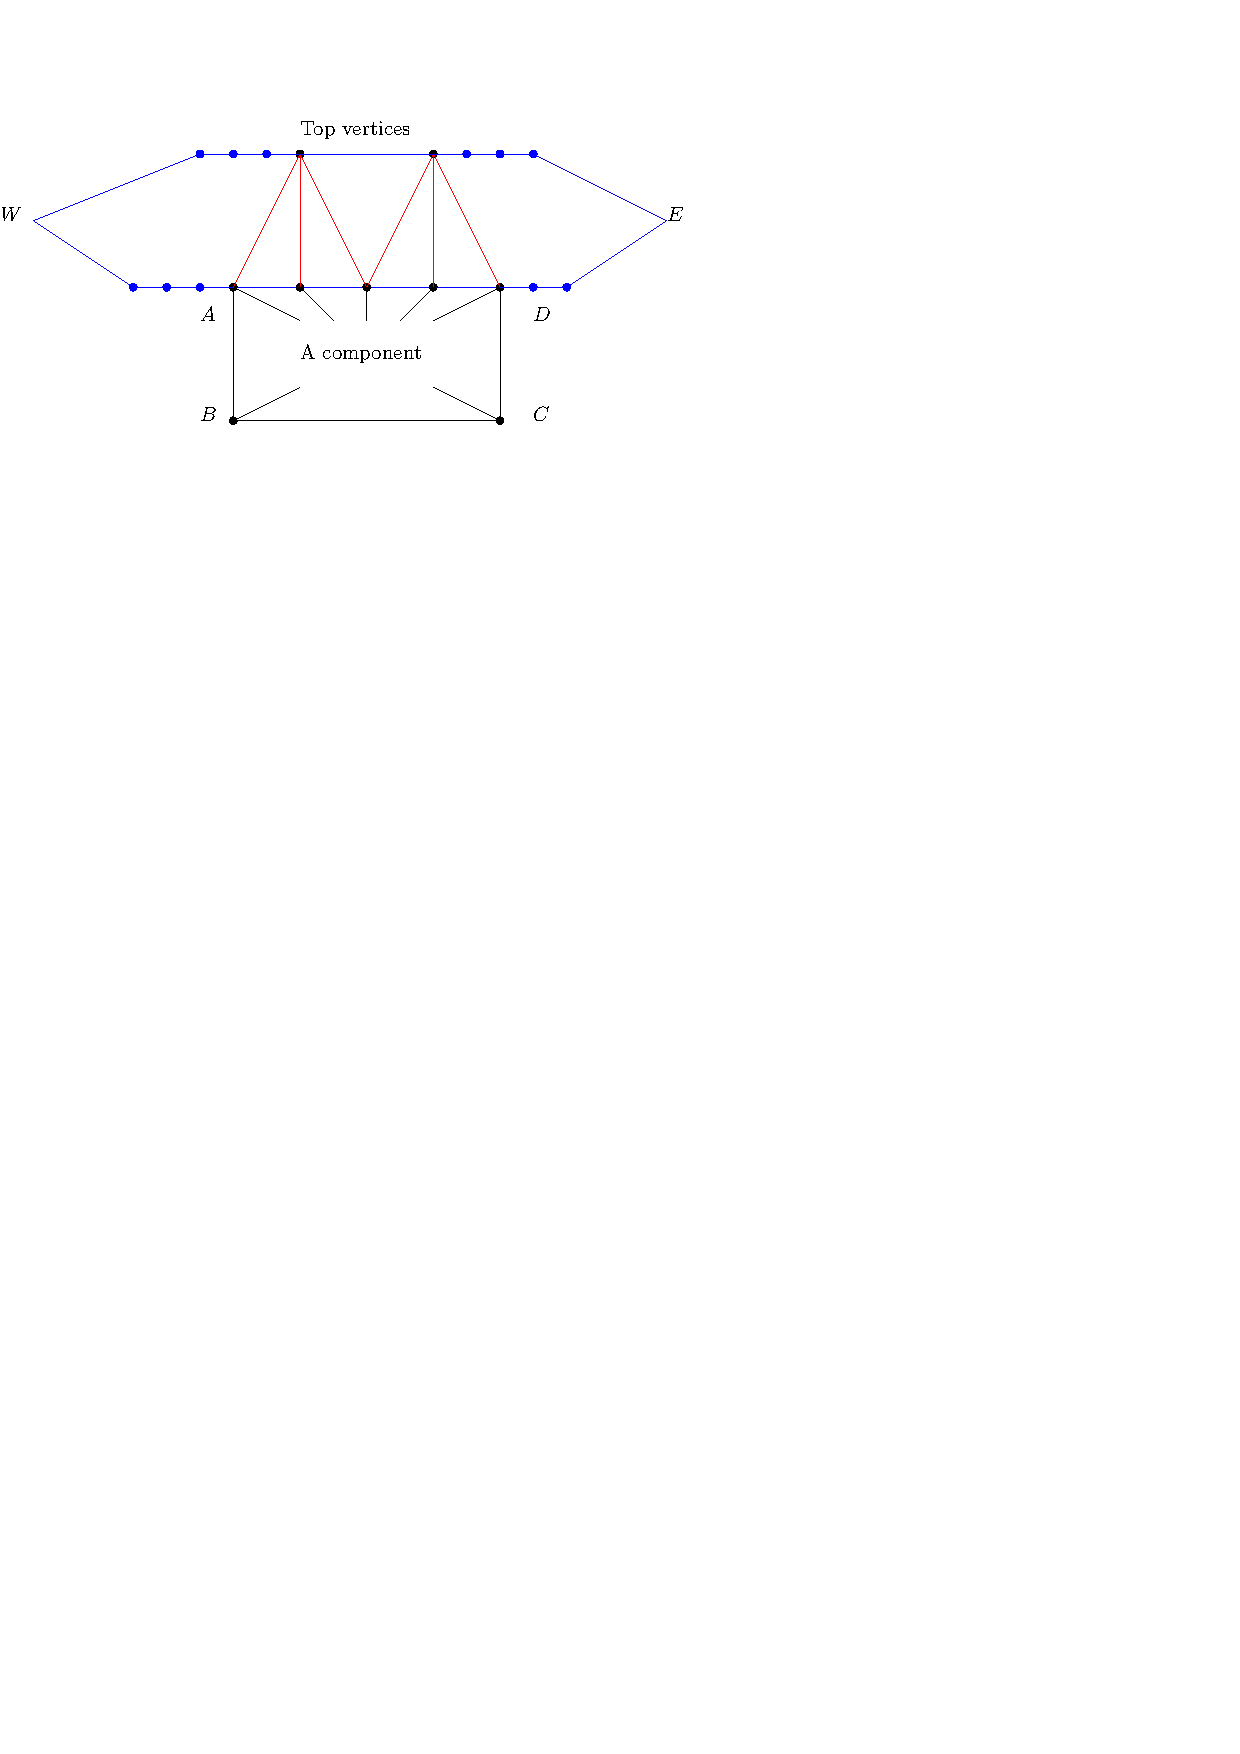
\includegraphics[scale=1]{chordShrink/img/situation}
  \caption{}
  \label{fig:chord:situation}
\end{figure}


We then shrink the entire interior of the bold \fxwarning{TODO} cycle to a single point and we arrive at the situation in Figure \ref{fig:chord:shrink}.

\begin{figure}[h]
  \centering
  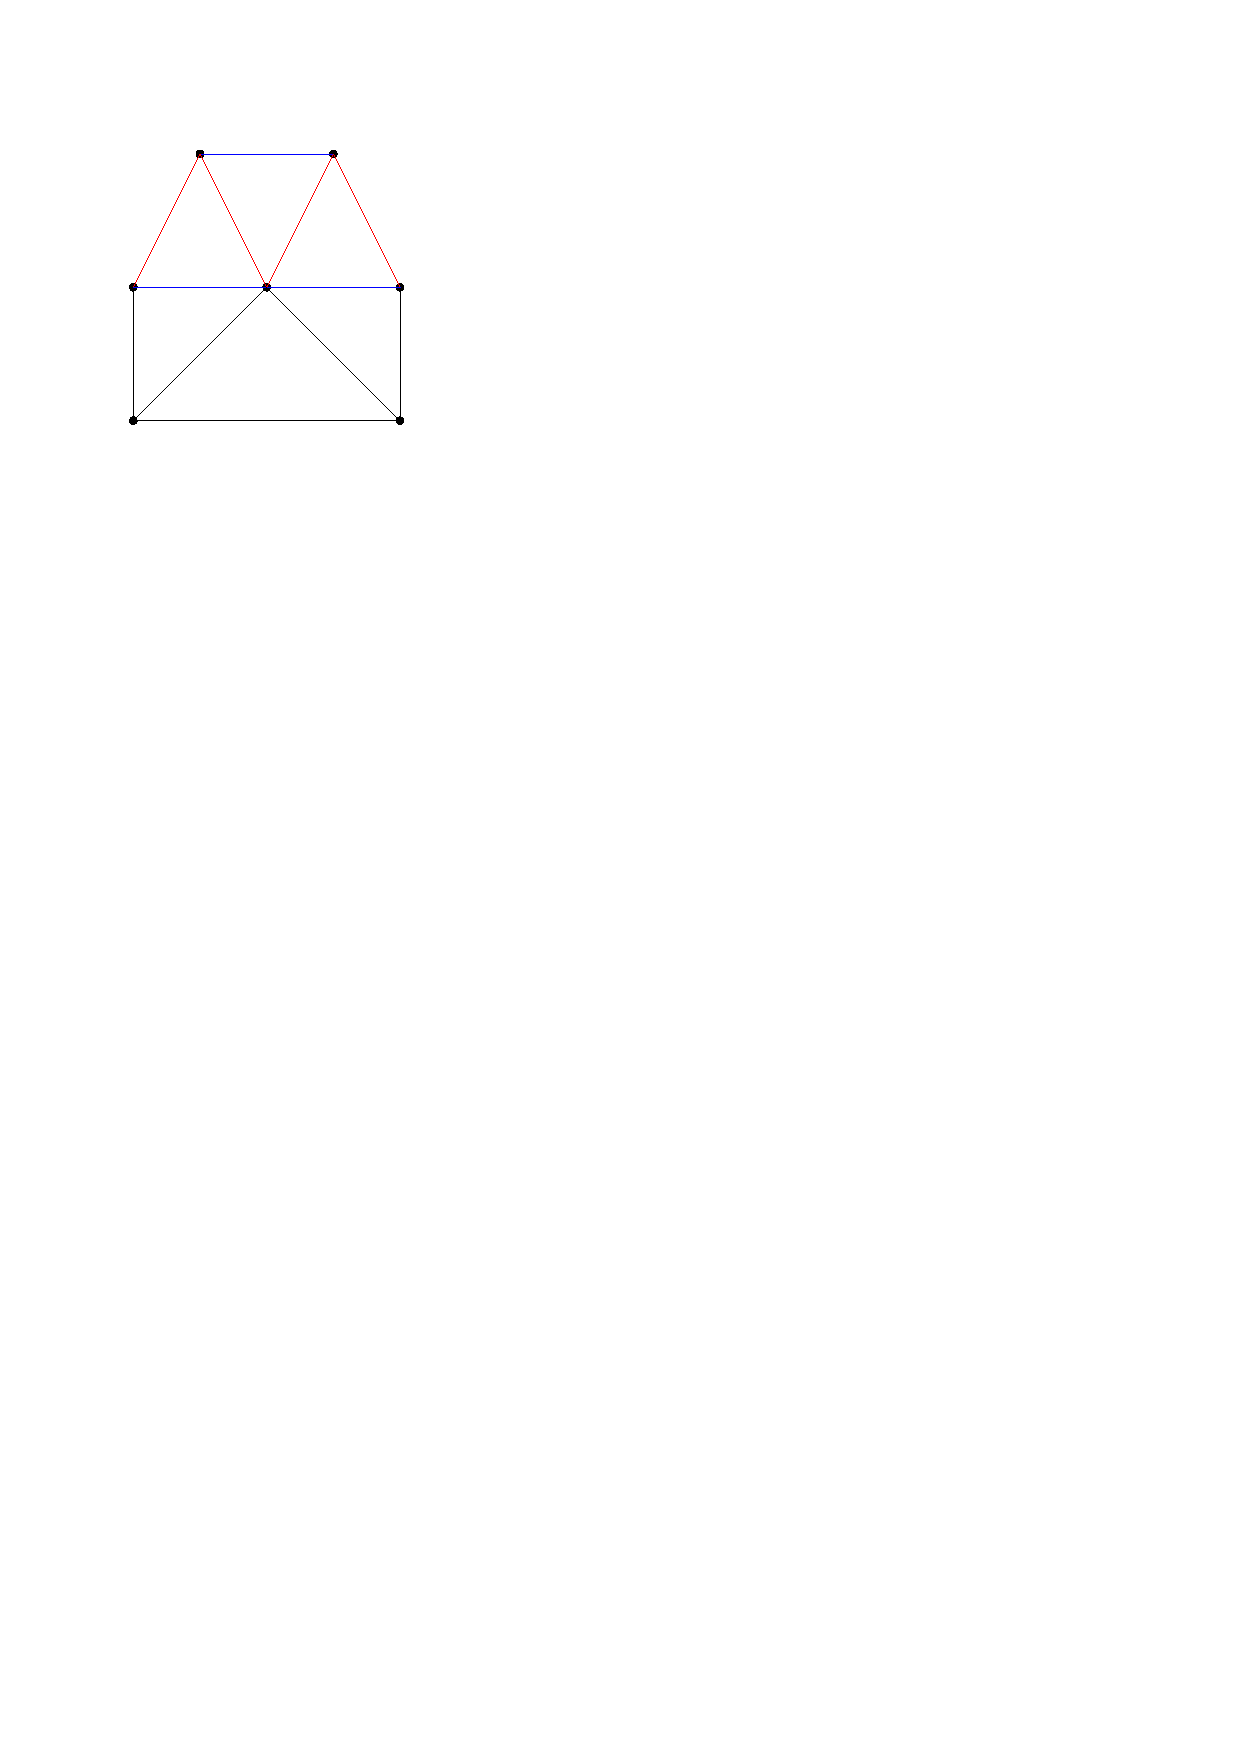
\includegraphics[scale=1]{chordShrink/img/shrink}
  \caption{Applying the shrink}
  \label{fig:chord:shrink}
\end{figure}

We always do this for a \emph{maximal} chord. That is a chord whose \emph{range} is not contained in the range of any other chord.

We then have the following Lemma's

\begin{lemma}
  \label{lm:}
  The shrink does not create a seperating triangle.
\end{lemma}

\begin{proof}
  A seperating triangle would be created if two nonadjecent vertices would be connceted by an edge.

  An conncetion between two topvertices would be an chord in an earlier valid path. This is forbidden. A conncetion between a top vertex and A, B, C or D Would also intersect a sweepline. Wich is imposible.

  An conncetion $AC$ or $BD$ would give a seperating $2-$chord on the sweepline. Which is something we avoid.

  Hence the shrink can't create a seperating triangle.
\end{proof}



\begin{lemma}
  \label{lm:}
  The shrink does not create any $4$-cycles that are wholly on or below the sweepcycle.
\end{lemma}

\begin{proof}
  Such an cycle $\C$ would be created by an 2 edge connection between $A$ and $C$, $B$ and $D$ or $A$ and $D$. The last one would imply a seperating 2-chord on the sweepcyle, so this can't be.

  The other two would imply a larger chord containing the chord $BC$. However we took the largest chord.
\end{proof}

Any 4-cycle partially above the 4-cycle doens't infuence the solvability of this graph badly. Since the part of the graph is above the sweepcycle is functionally the same as a large North vertex. \fxwarning{TODO Make this rigorous?}

More rigorously we could show that these things don't affect or possibility to find new valid paths.
